\documentclass{beamer}
%\usepackage{fullpage}
%\usepackage[left=2.8cm,right=2.2cm,top=2 cm,bottom=2 cm]{geometry}
\setbeamersize{text margin left=10pt,text margin right=10pt}
\usepackage{amsmath,amssymb}             % AMS Math
\usepackage[T1]{fontenc}
\usepackage[utf8]{inputenc}
\usepackage[french,english]{babel}
\usepackage{txfonts} 
\usepackage[]{graphicx}
\usepackage{multirow}
\usepackage{hyperref}
\usepackage{verbatim}
\usepackage{multicol}

%\renewcommand{\baselinestretch}{1.5}

\def\supit#1{\raisebox{0.8ex}{\small\it #1}\hspace{0.05em}}

\title[Towards improving automatic text summaries \hspace*{2cm}  \textbf{\footnotesize  \insertframenumber/\inserttotalframenumber} ] %
{Towards improving automatic text summaries \\ {\scriptsize Vers une amélioration des résumés automatiques de textes}}
\institute{ %
École  nationale Supérieure d'Informatique (ESI, ex. INI), Algérie  %\\\supit{b} CERIST - Algérie %
}
\author[Abdelkrime ARIES  (ESI 2016)] %
{Abdelkrime ARIES\\ {\footnotesize %
Supervisors: Pr. Zegour \& Pr. Hidouci \\
Research Group: D3 Team}}

\titlegraphic{
\includegraphics[height=1cm]{IMG/esi-logo.png}%\hspace*{4.75cm}~
}

\date{LCSI laboratory mid-term seminars: April 19th, 2016} %\today

\usetheme{Warsaw} % Antibes Boadilla Warsaw

\beamertemplatenavigationsymbolsempty


\begin{document}

\selectlanguage {francais}

\begin{frame}[plain]
\maketitle
\end{frame}


\begin{frame}
\frametitle{Plan}
{\footnotesize \tableofcontents[hideothersubsections]}
\end{frame}

\section{Problematic}

\begin{frame}
\begin{center}
{\Huge Problematic}
\end{center}
\end{frame}

\subsection{Motivation}

\begin{frame}
\frametitle{Problematic}
\framesubtitle{Motivation}

Why should we summarize?
\begin{center}
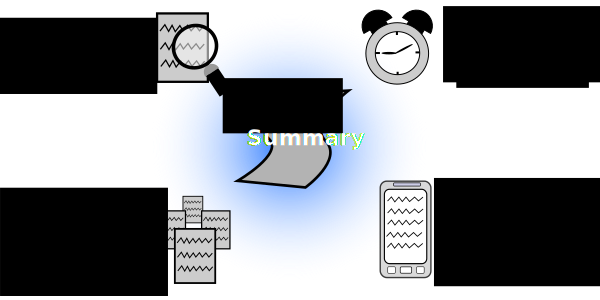
\includegraphics[height=6cm]{IMG/sum-benefit.pdf}
\end{center}

\end{frame}

\subsection{Summarization classification}

\begin{frame}
\frametitle{Introduction}
\framesubtitle{Summarization classification}
Following \cite{98-hovy-lin,99-sparckjones}:
\begin{center}
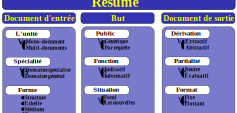
\includegraphics[width=10cm]{IMG/sum-classif.pdf}
\end{center}
\end{frame}

\subsection{Extractive vs. Abstractive}

\begin{frame}
\frametitle{Problematic}
\framesubtitle{Extractive vs. Abstractive}

Extractive:\\
\begin{itemize}
\item + Fast with less resources (CPU + data)
\item + Can be simply applied to many languages (statistical)
\item - Incoherent text
\item - Just pertinent sentences which can have no relation between them
\end{itemize}

Abstractive:\\
\begin{itemize}
\item + Good text presentation
\item + Redundancy can be dealt with
\item - Slow with a lot of resources (CPU + data)
\item - Hard to be implemented (language dependent)
\end{itemize}

\end{frame}

\subsection{Multi-Lingual systems}

\begin{frame}
\frametitle{Problematic}
\framesubtitle{Multi-Lingual systems}

\begin{itemize}
\item Process more than one language.
\item Language independent application:
\begin{itemize}
\item Fully independent 
\item Partial independent 
\end{itemize}
\end{itemize}
\vfill
Also, there are \textbf{Cross-lingual} systems

\end{frame}

\subsection{Objectives}
\begin{frame}
\frametitle{Problematic}
\framesubtitle{Objectives}

\begin{itemize}
\item Create a multi-lingual system.
\item Introduce abstractive 
\item Improve our method \cite{13-aries-al}.
\item Improve readability and coherence.
\end{itemize}
\end{frame}

\section{Extractive methods}

\begin{frame}
\begin{center}
{\Huge Extractive methods}
\vfill
{\Huge AllSummarizer as example}
\end{center}
\end{frame}

\subsection{AllSummarizer}
\begin{frame}
\frametitle{Extractive methods}
\framesubtitle{AllSummarizer}

\begin{center}
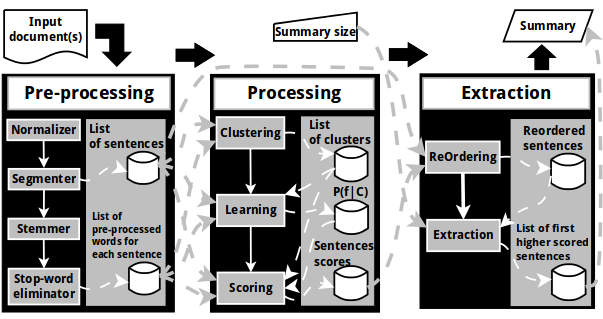
\includegraphics[width=100mm]{IMG/gnrl-arch.pdf}
\end{center}

\end{frame}

\subsection{Amelioration}
\begin{frame}
\frametitle{Extractive methods}
\framesubtitle{Amelioration}
Some ameliorations have been made to the original AllSummarizer system \cite{13-aries-al}:

\begin{enumerate}

\item Adding more features to the Unigram and Bigram term frequencies:
\begin{itemize}
\item Sentence position
\item Sentence length with stop words.
\item Sentence length without stop words.
\end{itemize}

\item Adding more languages to the preprocessing task (27 languages): 
Arabic, Bulgarian, Catalan, Czech, German, Greek, English, Spanish, Basque, Persian, Finnish, French, Hebrew, Hindi, Hungarian, Indonesian, Italian, Japanese, Dutch, Nynorsk, Norwegian, Portuguese, Romanian, Russian, Swedish, Thai, Turkish and Chinese. 

\end{enumerate}

\end{frame}

\begin{frame}
\frametitle{Extractive methods}
\framesubtitle{Amelioration}

\begin{enumerate}
\setcounter{enumi}{2}

\item Testing the summarizer with more than 40 languages (we used default preprocessing for languages without a preprocessing task).

\item Fixing the problem of redundant sentences (especially in case of multi-document summarization). 
This was done by calculating the similarity between the last added sentence and the sentence to be added. 
Then judging if they are similar using clustering threshold.

\item Estimating the threshold and the features for each language (multi and single document summarization). 
For more information, see our participation in MultiLing2015 workshop (SIGDIAL conference) \cite{15-aries-al}.

\end{enumerate}

\end{frame}

\subsection{Links}
\begin{frame}
\frametitle{Extractive methods}
\framesubtitle{Links}

Take a look: \\
\url{https://github.com/kariminf/AllSummarizer} \\
\vfill
Test it: \\
\url{allsummarizer-kariminf.rhcloud.com} 

\end{frame}

\section{Abstractive methods}

\begin{frame}
\begin{center}
{\Huge Abstractive methods}
\vfill
{\Huge Our vision}
\end{center}
\end{frame}

\subsection{Our vision}
\begin{frame}
\frametitle{Abstractive methods}
\framesubtitle{Our vision}

\begin{center}
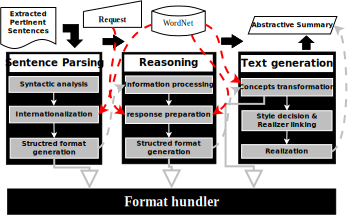
\includegraphics[width=100mm]{IMG/abs-arch.pdf}
\end{center}

\end{frame}

\subsection{Format handler}
\begin{frame}
\frametitle{Abstractive methods}
\framesubtitle{Format handler}

To communicate information between sentences, we proposed a new format called STON (``Sentence object notation").

\begin{itemize}
\item Represent sentences morphological and syntactic characteristics in a multi-lingual way.
\end{itemize}

Take a look:\\
\url{https://github.com/kariminf/SentRep}


\end{frame}

\begin{frame}
\frametitle{Abstractive methods}
\framesubtitle{Format handler}

{\LARGE \textbf{Format:}}\\

\begin{itemize}
\item Roles: each entity has a role to play in the clause (or sentence); It can be a subject, object, place, time, etc.
\item Actions: actions are the dynamic part in a clause, they link roles.
\item Sentences: Role-Action model can't represent every information. 
for instance, successive actions have to be represented somewhere.
\end{itemize}

\end{frame}

\begin{frame}[fragile]
\frametitle{Abstractive methods}
\framesubtitle{Format handler}

{\LARGE \textbf{Example:}}
Mother stayed at home.\\
\begin{multicols}{3}
\scriptsize\bf
\begin{verbatim}
@r: [
   r:{
      id: mother;
      syn: 10332385;
   r:}
   r:{
      id: home;
      syn: 3259505;
   r:}
r:]




@act: [
      act:{
         id: stay;
         syn: 117985;
         tense: PA;
         subj: [mother];
         @rel:[
            rel:{
               type: P_PLACE;
               ref: [home];
            rel:}
         rel:]
      act:}
act:]

@st: [
   st:{
      type: AFF;
      act: [stay];
   st:}
st:]







\end{verbatim}
\end{multicols}

\end{frame}


\subsection{Sentence Parsing}
\begin{frame}
\frametitle{Abstractive methods}
\framesubtitle{Sentence Parsing}

Working on it ... \\

\begin{itemize}
\item For now, we code an English2Ston parser.
\item Syntactic analysis (English): Stanford parser.
\item To this day, we just can parse sentences in the form : \\
"Subject\{simple singular\} Verb\{past, present simple\} Object\{simple singular\}". 
\end{itemize}
\vfill
Take a look:\\
\url{https://github.com/kariminf/NaLanPar}

\end{frame}

\subsection{Reasoning}
\begin{frame}
\frametitle{Abstractive methods}
\framesubtitle{Reasoning}

Our aim: \\
\begin{itemize}
\item Thoughts are language-independent.
\item Mind contains many thoughts.
\item People has thoughts about what others think.
\item Thoughts have truth level: belief, thinking, fact, etc. 
\end{itemize}
\vfill
So ... Will be presented Next time

\end{frame}


\subsection{Text generation}
\begin{frame}
\frametitle{Abstractive methods}
\framesubtitle{Text generation}

Working on it ... \\

\begin{itemize}
\item For now, we code an Ston2English, Ston2French generator.
\item Sentence Realization (English, French): SimpleNLG-EnFr.
\item To this day, we just can parse sentences in the form : "Subject\{simple singular\} Verb\{past, present simple\} Object\{simple singular\}". 
\end{itemize}
\vfill
Take a look:\\
\url{https://github.com/kariminf/NaLanGen}

\end{frame}

\section{Demo}
\begin{frame}
\frametitle{Demo}

\begin{center}
{\Huge Demonstration}
\end{center}

\end{frame}

%=======================END========================
\section{Thank you}
\begin{frame}
\frametitle{So ...}

\begin{center}
{\huge Less has been done, more to be done}
\vfill
{\LARGE Always remember:}
\\
{\Huge Summarizing saves time}
\end{center}

\end{frame}


%\subsection{Bibliography}
\frame[allowframebreaks]%
{\frametitle{Bibliography}
\tiny
\bibliography{biblio}
\bibliographystyle{IEEEtran} 
}


\end{document}

